\chapter{Methods}
\label{ch:methods}

\section{Laboratory methods}
\label{sec:methods-lab}

\subsection{Strains and media}
\label{subsec:methods-strains_media}

The \textit{Saccharomyces cerevisiae} strains used in this thesis are described in Table~\ref{tab:methods-strains}.

\begin{table}[hb]
  \footnotesize
  \centering
  \begin{tabularx}{\linewidth}{bbbbb}
    \toprule
    Name & Background & Genotype & Origin & Notes\\
    \midrule
    FY4 & FY4 & --- & EUROSCARF & \textcite{winstonConstructionSetConvenient1995} \\
    htb2::mCherry & FY4 & HTB2::mCherry & In-house, CRISPR & --- \\
    BY4741 & BY4741 & \textit{MAT}a \textit{his3$\Delta$1 leu2$\Delta$0 met15$\Delta$0 ura3$\Delta$0} & EUROSCARF & \textcite{brachmannDesignerDeletionStrains1998}\\
    \textit{zwf1$\Delta$} & BY4741 & \textit{zwf1$\Delta$::KAN} & Edinburgh Genome Foundry & Yeast deletion collection \\
    BY4742 & BY4742 & \textit{MAT}$\alpha$ \textit{his3$\Delta$1 leu2$\Delta$0 lys2$\Delta$0 ura3$\Delta$0} & Bruce Morgan & \textcite{calabreseHyperoxidationMitochondrialPeroxiredoxin2019}\\
    \textit{tsa1$\Delta$ tsa2$\Delta$} & BY4742 & \textit{tsa1$\Delta$::natNT2 tsa2$\Delta$::kanMX4} & Bruce Morgan & \textcite{calabreseHyperoxidationMitochondrialPeroxiredoxin2019} \\
    CEN.PK113-7D & CEN.PK113-7D & --- & Peter K\"{o}tter & \textcite{nijkampNovoSequencingAssembly2012} \\
    \bottomrule \\
  \end{tabularx}
  \caption{Strains used in this thesis.}
  \label{tab:methods-strains}
\end{table}

The minimal medium described by \textcite{verduynEffectBenzoicAcid1992} was used unless otherwise stated.
This minimal medium does not contain riboflavin, thus minimising its effect on flavin autofluorescence imaging, and its composition is known and easily controlled.
Specifically, the composition of the carbon source-limiting medium is described in Tables~\ref{tab:methods-media-delft}--\ref{tab:methods-media-delft-vitamins}, and the media pH was adjusted to 6.0 using potassium hydroxide, or sodium hydroxide for potassium-free media.

\begin{table}[h]
  \footnotesize
  \centering
  \begin{tabularx}{\linewidth}{bbb}
    \toprule
    Reagent & Concentration & Remarks\\
    \midrule
    \ce{KH2PO4} & \SI{3.}{\gram~\litre^{-1}} & \\
    \ce{MgSO4.7H2O} & \SI{0.5}{\gram~\litre^{-1}} & \\
    \ce{(NH4)2SO4} & \SI{5.}{\gram~\litre^{-1}} & \\
    \ce{Trace metals} & \SI{1.}{\milli\litre~\litre^{-1}} & See Table~\ref{tab:methods-media-delft-metals} \\
    \ce{Vitamins} & \SI{1.}{\milli\litre~\litre^{-1}} & See Table~\ref{tab:methods-media-delft-vitamins}.  Add upon use. \\
    \ce{Carbon source} & variable & Add upon use. \\
    \bottomrule \\
  \end{tabularx}
  \caption[
    Composition of base minimal medium
  ]{
    Composition of base minimal medium.
    For potassium-free media, replace \ce{KH2PO4} with \SI{2.65}{\gram~\litre^{-1}} \ce{NaH2PO4}, which gives the same molarity.
  }
  \label{tab:methods-media-delft}
\end{table}

\begin{table}[h]
  \footnotesize
  \centering
  \begin{tabularx}{\linewidth}{bbS}
    \toprule
    Reagent & Formula & {Concentration [\SI{}{\gram~\litre^{-1}}]}\\
    \midrule
    EDTA & \ce{C10H14N2Na2O8.2H2O} & 15.00 \\
    Zinc sulfate & \ce{ZnSO4.7H2O} & 4.50 \\
    Manganese (II) chloride & \ce{MnCl2.2H2O} & 0.84 \\
    Cobalt (II) chloride & \ce{CoCl2.6H2O} & 0.30 \\
    Copper (II) sulfate & \ce{CuSO4.5H2O} & 0.30 \\
    Sodium molybdate & \ce{Na2MoO4.2H2O} & 0.40 \\
    Calcium chloride & \ce{CaCl2.2H2O} & 4.50 \\
    Iron (II) sulfate & \ce{FeSO4.7H2O} & 3.00 \\
    Boric acid & \ce{H3BO3} & 1.00 \\
    Potassium iodide & \ce{KI} & 0.10 \\
    \bottomrule \\
  \end{tabularx}
  \caption[
    Composition of trace metal mix
  ]{
    Composition of trace metal mix for minimal media described in Table~\ref{tab:methods-media-delft}.
  }
  \label{tab:methods-media-delft-metals}
\end{table}

\begin{table}[h]
  \footnotesize
  \centering
  \begin{tabularx}{\linewidth}{bbS}
    \toprule
    Reagent & Formula & {Concentration [\SI{}{\gram~\litre^{-1}}]}\\
    \midrule
    D-(+)-biotin & \ce{C10H16N2O3S} & 0.05 \\
    D-panthothenic acid calcium salt & \ce{Ca(C9H16NO5)2} & 1.00 \\
    Nicotinic acid & \ce{C6H5NO2} & 1.00 \\
    \textit{myo}-Inositol & \ce{C6H12O6} & 25.00 \\
    Thiamine chloride hydrochloride & \ce{C12H15ClN4OS.HCl} & 1.00 \\
    Pyridoxal hydrochloride & \ce{C8H12ClNO3} & 1.00 \\
    4-aminobenzoic acid & \ce{C7H7NO2} & 0.20 \\
    \bottomrule \\
  \end{tabularx}
  \caption[
    Composition of vitamin mix
  ]{
    Composition of vitamin mix for minimal media described in Table~\ref{tab:methods-media-delft}.
  }
  \label{tab:methods-media-delft-vitamins}
\end{table}

For auxotrophic strains, supplements were added according to Table~\ref{tab:methods-media-auxotroph}.
Then, a carbon source is added as appropriate to create the growth medium.

\begin{table}[h]
  \footnotesize
  \centering
  \begin{tabularx}{\linewidth}{bS}
    \toprule
    Reagent & {Concentration [\SI{}{\milli\gram~\litre^{-1}}]} \\
    \midrule
    histidine & 125. \\
    leucine & 500. \\
    tryptophan & 75. \\
    methionine & 100. \\
    uracil & 150. \\
    \bottomrule \\
  \end{tabularx}
  \caption[
    Supplements to minimal media for auxotrophic strains
  ]{
    Supplements to minimal media for BY4741-background auxotrophic strains, compositions derived from \textcite{pronkAuxotrophicYeastStrains2002}.
    For BY4742-background strains, replace methionine with \SI{100}{\milli\gram~\litre^{-1}} lysine-HCl.
  }
  \label{tab:methods-media-auxotroph}
\end{table}

\subsection{Single-cell microfluidics}
\label{subsec:methods-microfluidics}

Cells were grown from colonies on solid agar in a liquid culture composed of minimal media formulation appropriate for the experiment, supplements appropriate for the strain's auxotrophy, and a carbon source (glucose or pyruvate) appropriate for the experiment (see Section~\ref{subsec:methods-strains_media}).
% Kevin's OD measurements?
The cells were incubated at \SI{30}{\celsius} for \SI{14}{\hour} (overnight) if the carbon source is glucose or \SI{48}{\hour} if the carbon source is pyruvate.
Subsequently, the cells were diluted so that the resulting culture had an OD\textsubscript{600} of 0.10--0.20, and were then incubated for a further \SI{4}{\hour}.

To monitor metabolic cycles in single cells, ALCATRAS microfluidics  \parencite{craneMicrofluidicSystemStudying2014} devices were prepared and connected to syringes containing nutrient media (Fig.\ \ref{fig:methods-chip}).
ALCATRAS microfluidic devices were made from polydimethylsiloxane (PDMS), with a 10:1 ratio between Sylgard 184 (Dow Corning) and curing agent.
The devices consist of chambers that contain of a dense array of cell traps to trap parent cells, allowing approximately 100 traps to be imaged at once using a 40 $\times$ objective lens magnification.

\begin{figure}
  \centering
  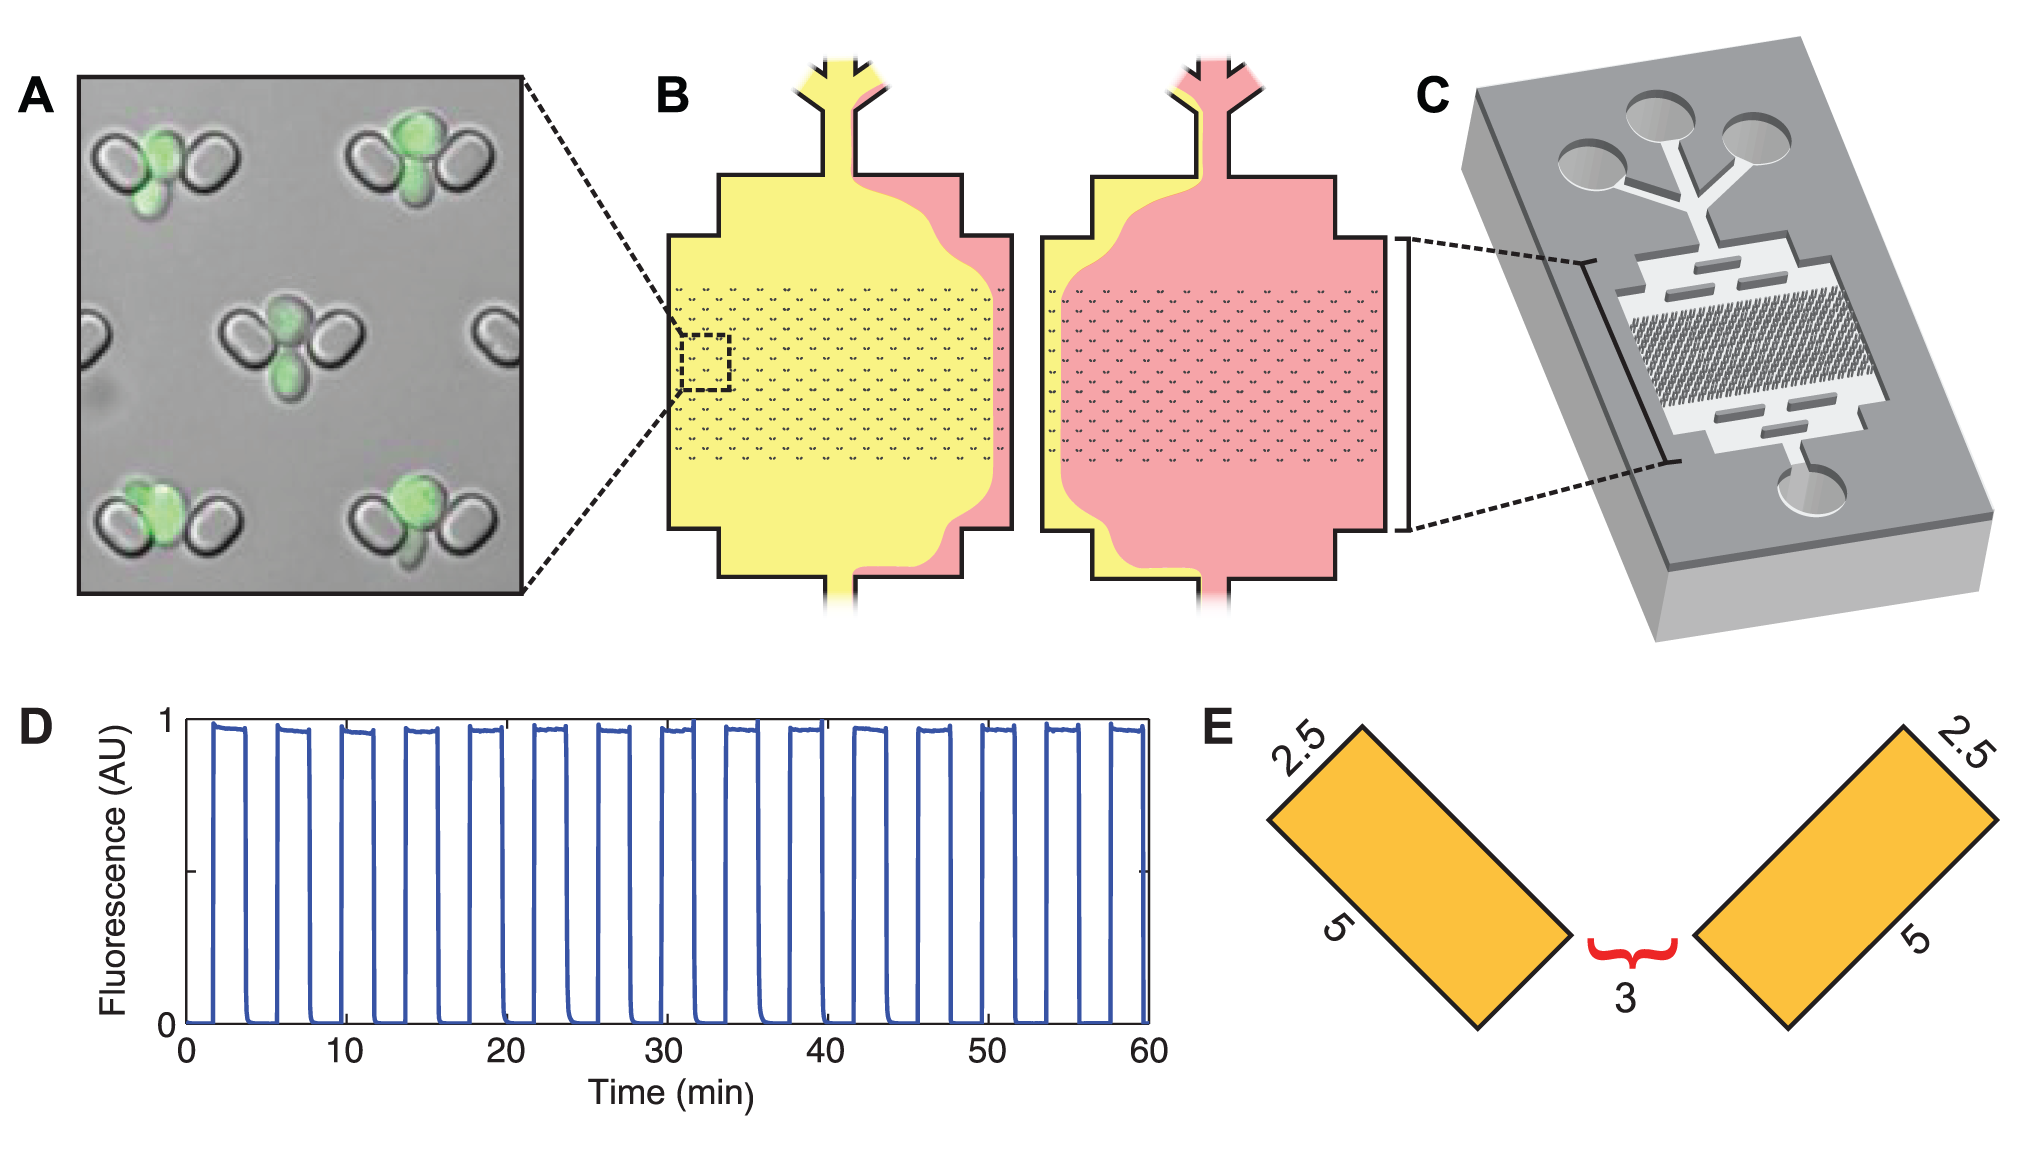
\includegraphics[width=0.9\textwidth]{craneMicrofluidicSystemStudying2014_1}
  \caption[
    Overview of ALCATRAS microfluidic chip design.
  ]{
    Overview of ALCATRAS microfluidic chip design.
    \textbf{(A)} Sample brightfield image of cell traps in the chip, overlaid with fluorescence image of Doa1p-GFP, to indicate cells (green).
    \textbf{(B)} Switching between media sources (yellow to pink) occurs within \SI{6}{\second}.
    \textbf{(C)} Microfluidic chip design.
    \textbf{(D)} Switching rate was assessed by imaging the fluorescence in the chamber whilst the input medium was switched between a non-fluorescent medium and medium containing 0.1\% fluorescein.
    \textbf{(E)} Trap dimensions, in micrometres.
    Adapted from \textcite{craneMicrofluidicSystemStudying2014}.
      }
  \label{fig:methods-chip}
\end{figure}

The pressure on the syringes were controlled automatically to achieve a constant \SI{4}{\micro\litre~\minute^{-1}} media flow, creating laminar flow.
The shape of the traps allows parent cells to be trapped in place, while progeny cells leave the trap after they bud from parent cells as nutrient medium flows across the device.
Specifically, when a cell falls into a trap, the local pressure gradient changes to create a low-energy pocket that keeps the cell trapped, as evidenced by a simulation of fluid dynamics given the device design (Fig.\ \ref{fig:methods-fluid_dynamics}).

\begin{figure}
  \centering
  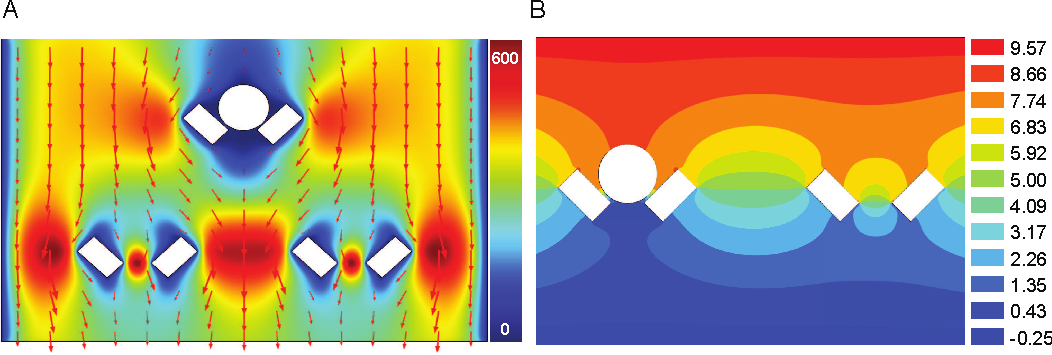
\includegraphics[width=0.9\textwidth]{craneMicrofluidicSystemStudying2014_S1}
  \caption[
    Fluid dynamic simulations of the ALCATRAS microfluic chip.
  ]{
    Fluid dynamic simulations of the ALCATRAS microfluic chip.
    \textbf{(A)} Velocity of fluid (in units of \SI{}{\micro\metre~\second^{-1}}) as a function of spatial position in the device.
    \textbf{(B)} Pressure of fluid (in units of \SI{}{\pascal}) as a function of spatial position in the device.
    Adapted from \textcite{craneMicrofluidicSystemStudying2014}.
      }
  \label{fig:methods-fluid_dynamics}
\end{figure}

PDMS is known to absorb small, hydrophobic molecules \parencite{toepkePDMSAbsorptionSmall2006}, and molecules with such properties are also known to adsorb onto the surface of PDMS \parencite{liPDMSCompoundAdsorption2009}.
These physical interactions decrease the effective concentration of such molecules in the nutrient media.
To decrease adsorption, a thin layer of silane was evaporated onto the wafer before moulding of PDMS devices \parencite{craneMicrofluidicSystemStudying2014}, and during experimental set-up, bovine serum albumin was added to create an additional coating on the internal surfaces of the microfluidic device.

To prepare for an experiment, a device's multiple chambers were filled with growth media supplemented with 0.05\% w/v bovine serum albumin, which was added to further decrease adsorption \parencite{toepkePDMSAbsorptionSmall2006}.
Cells were then loaded into the ALCATRAS chambers --- different chambers can house cells from different strains (Fig.\ \ref{fig:methods-microfluidics}).
% Syringe pumps containing media were programmed to produce a constant flow of \SI{4}{\micro\litre~\hour^{-1}} into the chambers.
% As a consequence, parent cells are held in place within traps, while progeny cells flow out of traps into the outflow after the parents bud.
There are two syringes that can contain different media, and in experiments that require different nutrient conditions at different times, the ALCATRAS system is programmed to switch between the two syringes.
The cells and ALCATRAS chambers were located in an incubation chamber (Oko-labs) that was maintained at \SI{30}{\celsius}.

\begin{figure}
  \centering
  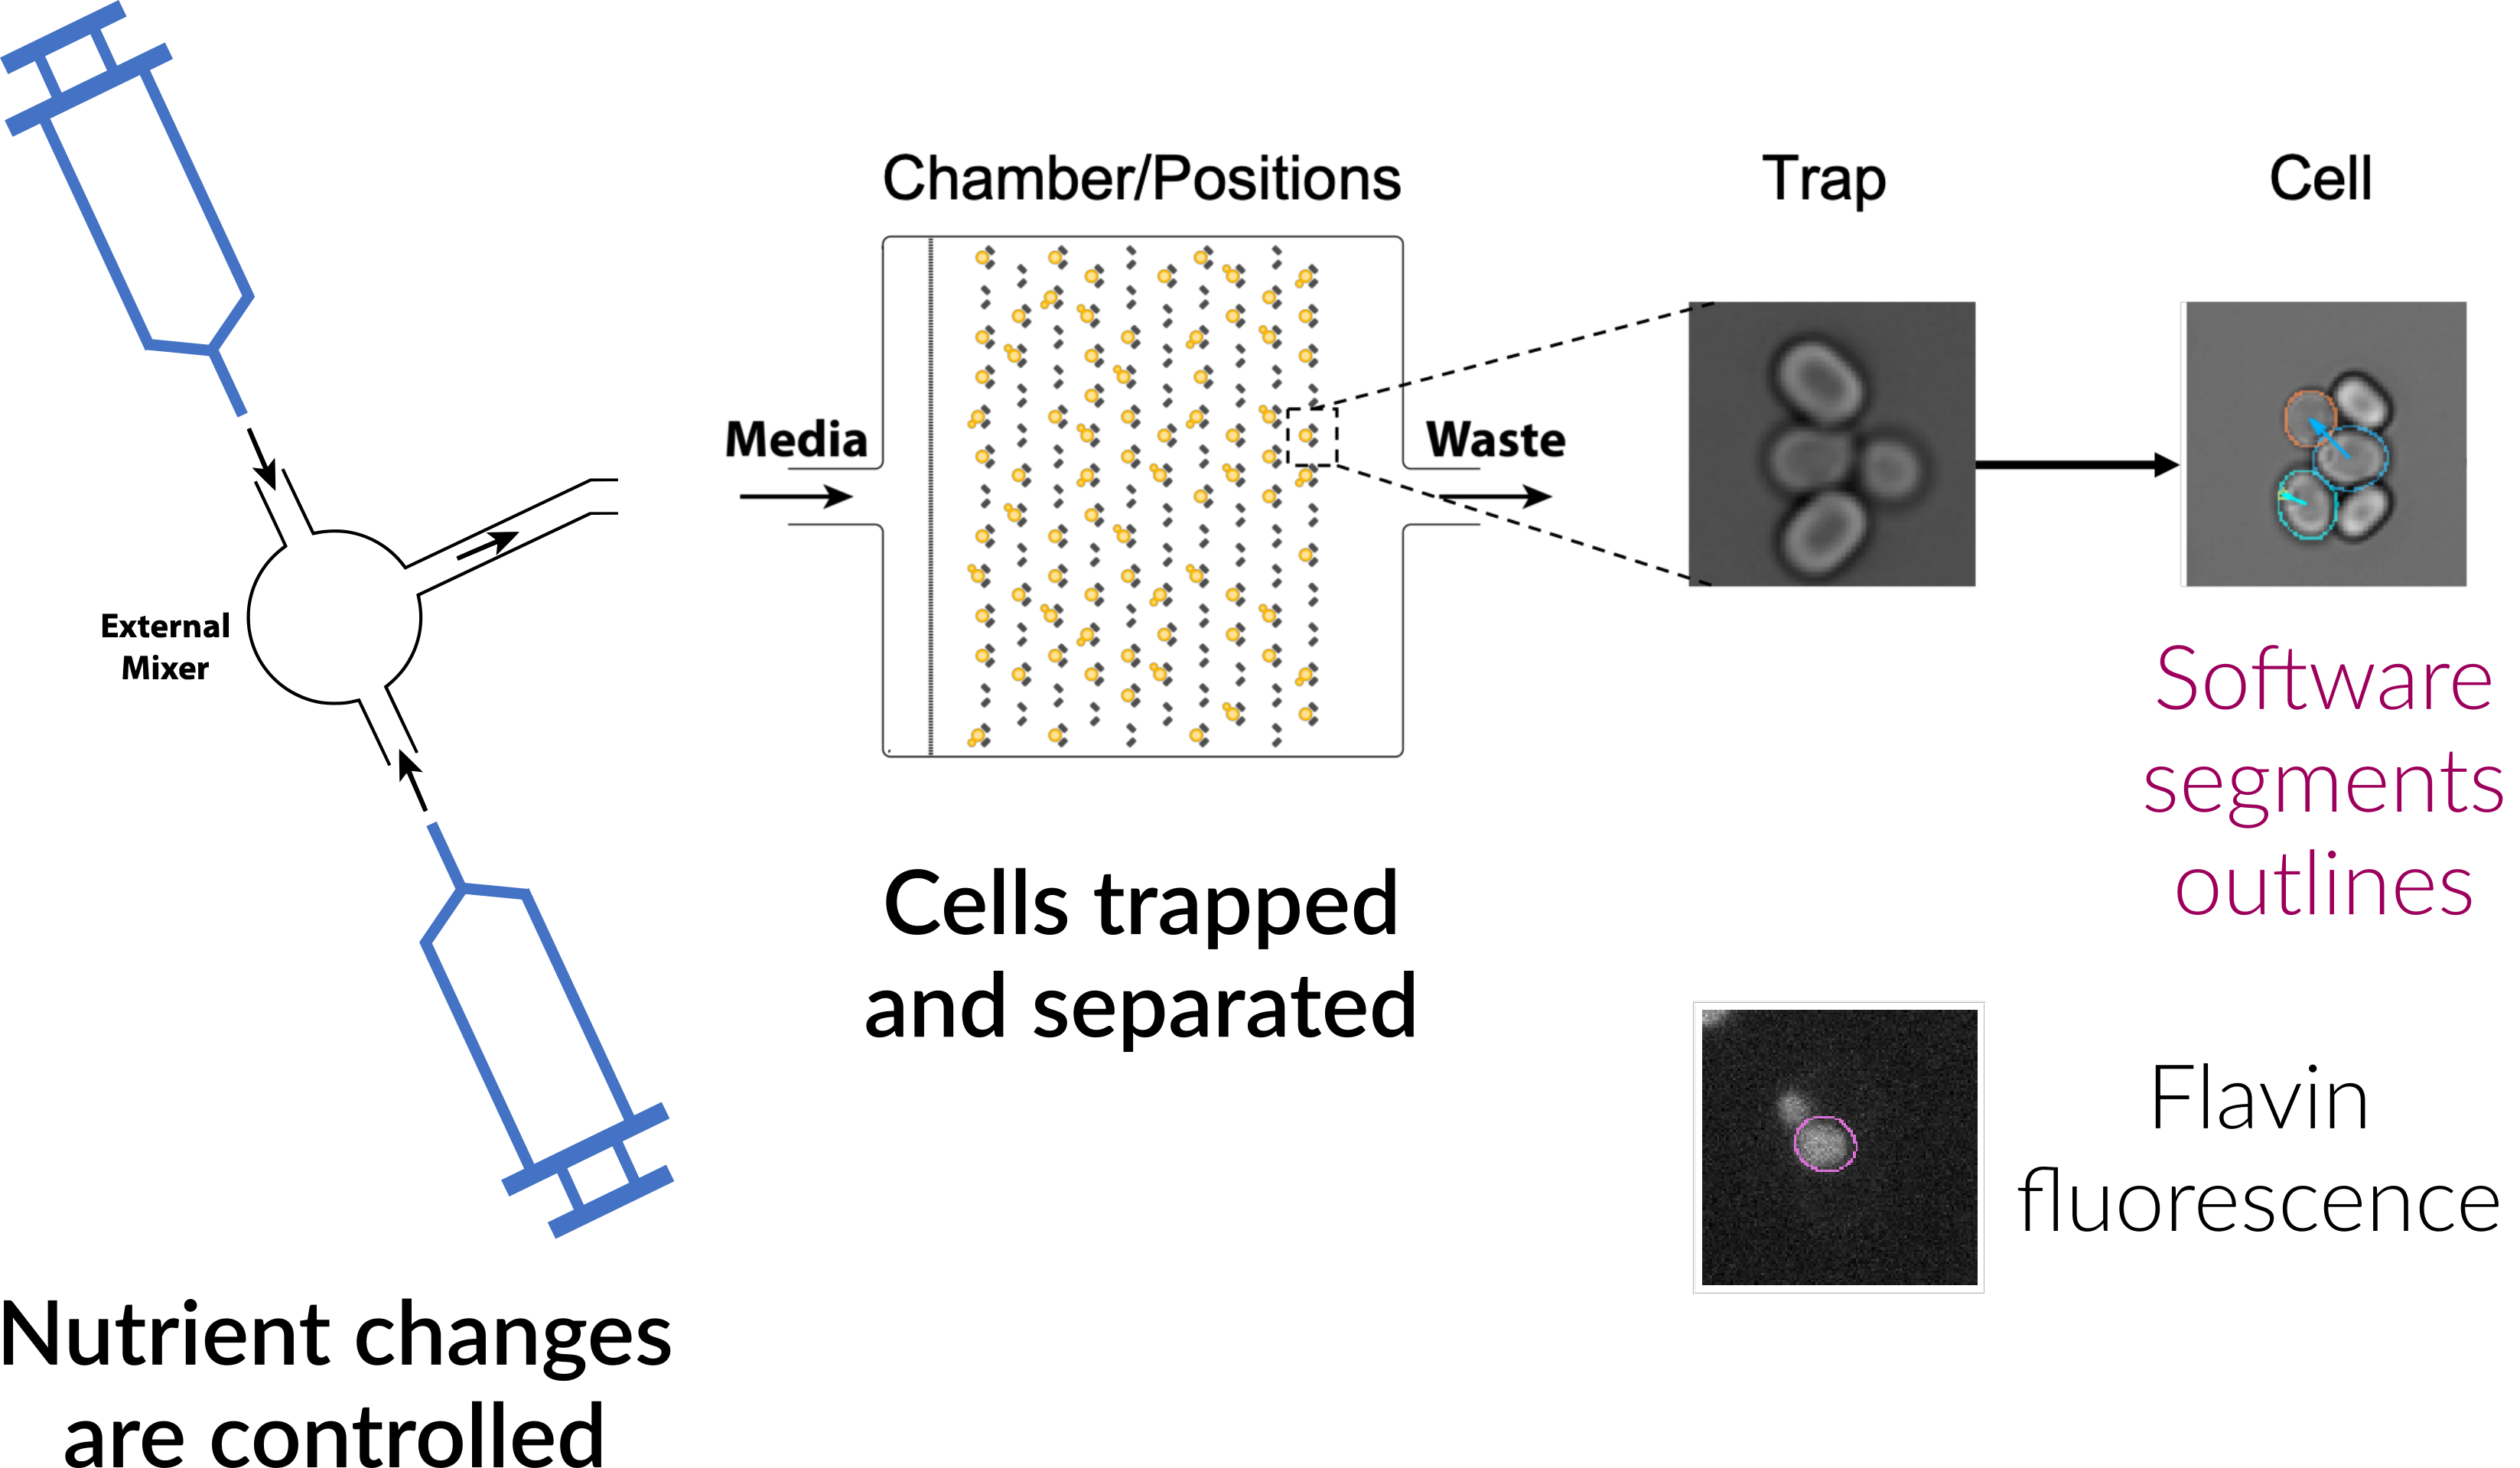
\includegraphics[width=0.9\textwidth]{microfluidics.png}
  \caption[
    Overview of single-cell microfluidics set-up using the ALCATRAS system
  ]{
    Overview of single-cell microfluidics set-up using the ALCATRAS system.
    Cells are loaded into chambers within devices, where they are trapped and separated (centre).
    The media composition the cells experience are controlled with syringe pumps (left).
    Brightfield and fluorescent images are taken at regular intervals, and then processed using \textit{aliby} \parencite{munozgonzalezPhenotypingSingleCells2023} to obtain time series of fluorescence intensity changes for each parent cell.
  }
  \label{fig:methods-microfluidics}
\end{figure}

Microscopy was performed using a 40 $\times$ 1.4 NA oil immersion objective (Nikon), and the Nikon Perfect Focus System was used to ensure consistent focus.
X-Y spatial positions were defined for each chamber to maximise spatial coverage of the chamber while ensuring that the microscope takes less time to move positions and capture images than the interval period.
Images were taken every \SI{5}{\minute}, and the duration of image acquisition varied for each experiment.
Brightfield and flavin images were captured in all strains and mCherry images were additionally captured for the HTB2::mCherry strain.
Five z-slices were taken for brightfield images, with a spacing of \SI{0.6}{\micro\metre} between slices.
Fluorescence imaging was performed with an OptoLED light source (Cairn Research), and LED voltage was optimised for maximum signal intensity without LED cut-off prior to experiments.
For flavin imaging, the excitation filter was set to 430/24 (\SIrange{418}{442}{\nano\metre}), the emission filter was set to 535/30 (\SIrange{520}{550}{\nano\metre}), and the exposure time was \SI{60}{\milli\second}.
One z-slice was taken for each flavin image in each position.
For mCherry imaging, the excitation filter was set to (\SIrange{555}{590}{\nano\metre}), the emission filter was to set to 632/60 (\SIrange{602}{682}{\nano\metre}) and the exposure time was \SI{100}{\milli\second}.
Five z-slices were taken for mCherry images, with a spacing of \SI{0.6}{\micro\metre} between slices.

\section{Image analysis methods}
\label{sec:methods-segmentation}

I used \textit{aliby} \parencite{munozgonzalezPhenotypingSingleCells2023}, an end-to-end Python-based software package developed for time-lapse microscopy, to process the microscope images in order to obtain flavin and mCherry time series for further analysis.

\textit{aliby} tracks tiles that correspond to a trap across time-lapse images to account for expected spatial drifting in the microscope.
It then uses \textit{BABY} \parencite{pietschDeterminingGrowthRates2023} to segment the images of traps to identify the outlines of cells and to track cells from one time point to another, creating a lineage of cells (Fig.\ \ref{fig:methods-timelapse}).
\textit{aliby} then overlays the cell outlines onto the fluorescence (flavin and mCherry) images to extract fluorescence intensity, and assigns a fluorescence value to each cell at each time point based on the mean intensity of pixels within the cell's outline.
The background fluorescence is also computed, based on the pixel intensity outside cell outlines, and is then subtracted from the cell fluorescence.

\begin{figure}[hp]
  \centering
  \begin{subfigure}[htpb]{0.6\textwidth}
   \centering
   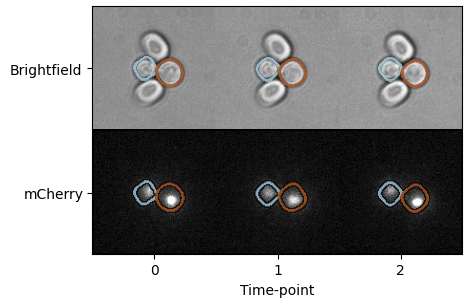
\includegraphics[width=\textwidth]{example_images_mCherry_edit.png}
   \caption{
   }
   \label{fig:methods-timelapse-images}
  \end{subfigure}

  \begin{subfigure}[htpb]{1.0\textwidth}
   \centering
   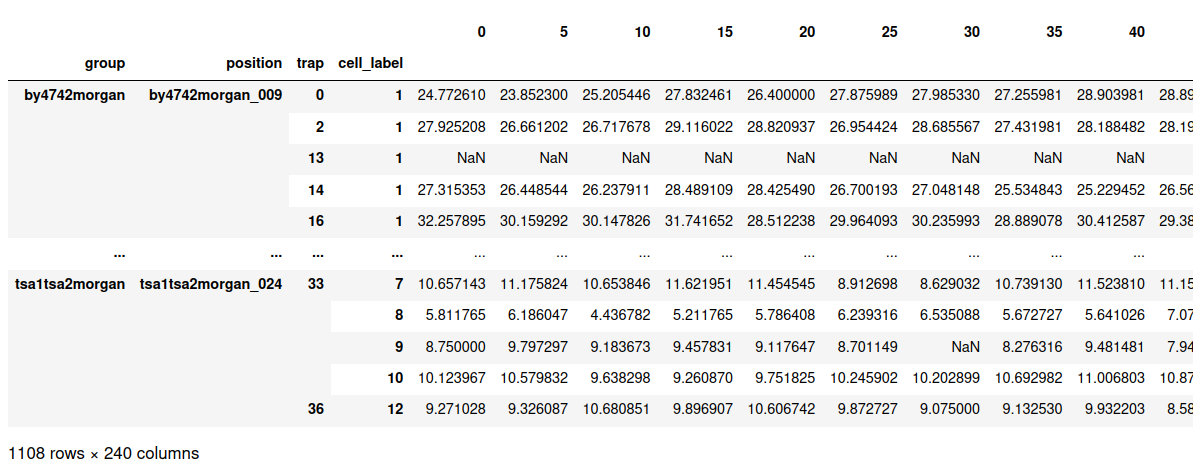
\includegraphics[width=\textwidth]{example_dataframe.png}
   \caption{
   }
   \label{fig:methods-timelapse-dataframe}
  \end{subfigure}

  \caption[
    Example time course of images from a microfluidics experiment, processed by \textit{aliby}.
    The extracted values were then saved in an array of numbers, with rows indicating cells (labelled by IDs) and columns indicating time in minutes --- each row thus represents a time series.
  ]{
    \textbf{(\ref{fig:methods-timelapse-images})}
    Example time course of images from a microfluidics experiment, processed by \textit{aliby} \parencite{munozgonzalezPhenotypingSingleCells2023}.
    Top row shows brightfield images taken over time; only the first three time points are shown for illustrative purposes.
    Here, \textit{BABY} \parencite{pietschDeterminingGrowthRates2023} segments brightfield images to obtain cell outlines (blue and brown).
    Bottom row shows images from a sample fluorescence channel taken over time.
    The cell outlines from image segmentation were overlaid onto the fluorescence channel images so that the fluorescence intensity within each cell can be extracted.
    \textbf{(\ref{fig:methods-timelapse-dataframe})}
    The extracted values were then saved in an array of numbers, with rows indicating cells (labelled by IDs) and columns indicating time in minutes --- each row thus represents a time series.
  }
  \label{fig:methods-timelapse}
\end{figure}

Flavin fluorescence thus represents the oxidation of flavins throughout the yeast metabolic cycle (see Section~\ref{sec:intro-flavin}), and mCherry fluorescence thus represents the amount of histone proteins as a proxy for cell division cycle progression \parencite{garmendia-torresMultipleInputsEnsure2018}.


\section{Time series analysis methods}
\label{sec:methods-computational}

\subsection{Data pre-processing}
\label{subsec:methods-computational-preprocessing}

To filter out long-term trends that may confound analysis of oscillatory time series, a high-pass Butterworth filter, with a critical frequency of \SI{2.86d-3}{\minute^{-1}}, corresponding to a period of \SI{350}{\minute}, was applied to fluorescence time series generated from \textit{aliby}.
% COMMENT TO PRESERVE ORIGINAL REF KEYS, AS OPPOSED TO RANGES SHOWN BELOW.
% TO BE PROPER, I CAN USE SMART REFS, BUT THEY ARE NOT IMPLEMENTED IN THIS THESIS.
% Specifically, Figs \ref{fig:biology-highglc-single}, \ref{fig:biology-highglc-sync-spectral}, \ref{fig:biology-highglc-sync-corr}, \ref{fig:biology-starvation}, \ref{fig:biology-by4741-sync}, \ref{fig:biology-cenpk-sync}, \ref{fig:biology-pyruvate}, \ref{fig:biology-lowglc}, \ref{fig:biology-compare-snr}, \ref{fig:biology-kdeficient}, \ref{fig:biology-kdeficient-snr}, \ref{fig:biology-zwf1}, and \ref{fig:biology-tsa1tsa2} in Chapter~\ref{ch:biology} and all figures from Chapter~\ref{ch:analysis} except for \ref{fig:analysis-filter-raw} are derived from filtered time series.
Specifically, Figs.\ \ref{fig:biology-highglc-single}, \ref{fig:biology-highglc-sync-spectral}--\ref{fig:biology-starvation}, \ref{fig:biology-by4741-sync}--\ref{fig:biology-lowglc}, \ref{fig:biology-compare-snr}, \ref{fig:biology-kdeficient}--\ref{fig:biology-kdeficient-snr}, and \ref{fig:biology-zwf1}--\ref{fig:biology-tsa1tsa2} in Chapter~\ref{ch:biology} and all figures from Chapter~\ref{ch:analysis} except for \ref{fig:analysis-filter-raw} are derived from filtered time series.
Section~\ref{sec:analysis-cleaning} further discusses the rationale for this filtering method.

However, the long-term shifts of fluorescence intensities are important for interpreting some results based on imposing temporary environmental perturbations on yeast cells.
In such cases, such long-term shifts would be filtered away by the high-pass Butterworth filter, and thus the filter was not applied.
Specifically, Figs.\ \ref{fig:biology-starvation-raw}--\ref{fig:biology-starvation-histogram}, and \ref{fig:biology-kdeficient-histogram} are derived from unfiltered time series.

\subsection{Classical periodogram}
\label{subsec:methods-computational-periodogram}

To detect rhythmicity in time series, I computed the periodogram, based on the classical (original) definition of the periodogram \parencite{schusterInvestigationHiddenPeriodicities1898,scargleStudiesAstronomicalTime1982}, and by using the fast Fourier transform, then used a statistical test for rhythmicity based on \textcite{glynnDetectingPeriodicPatterns2006}, described as follows:

\begin{enumerate}
\item Let the data have $\mathcal{G}$ cells.
Let cell $g = 1, \dots{}, \mathcal{G}$ have a time series with $N_{g}$ time points.
The time series is thus denoted $Y_{g}(t) = y_{g}(t_{1}), \dots{}, y_{g}(t_{N_{g}})$.
\item For each time series, I define a range of test frequencies linearly from $\frac{1}{N_{g}}$ to the Nyquist limit (i.e.\ half the rate of image acquisition).

With this definition, I compute the classical periodogram for each time series, via the Fourier transform:
  \begin{equation}
    P_{g}(\omega) = \frac{N_{g}}{2\sigma^{2}} \left|\int_{-\infty}^{\infty} Y_{g} e^{-2\pi it}dt \right|, % check constants, etc
    \label{eq:normalised-periodogram-ar}
  \end{equation}
        where $\sigma^{2}$ is the sample variance of $Y_{g}$.
        In this equation, the periodogram is normalised by the coefficient $N_{g}/2\sigma^{2}$ so that the area under the periodogram is constant across all time series.
        The Lomb-Scargle periodogram is equivalent to the classical periodogram if the time points are equally spaced \parencite{lombLeastsquaresFrequencyAnalysis1976}, as is the case for the vast majority of my data.
  \item For each cell $g$, I denote the peak $h_{g} = \max_{j}P_{g}(\omega)$.
        The peak of the normalised classical periodogram of each time series was used as a proxy for the quality of oscillation.
  \item I define an effective number of independent frequencies $M = f_{max}N_{g}$ for each time series, where $f_{max}$ is the Nyquist limit \parencite{vanderplasUnderstandingLombScarglePeriodogram2018}.
  I then calculate the $p$-value of testing the null hypothesis that such a peak is due to chance:
  \begin{equation}
    p_{g} = 1 - {(1 - e^{-h_{g}})}^M
    \label{eq:lsp-pval}
  \end{equation}
  This formula is based on the exponential distribution of the power at a given frequency in the periodogram \parencite{scargleStudiesAstronomicalTime1982}.
\item I order the cells by $p$-values: $p_{1} \leq p_{2} \leq \cdots \leq p_{\mathcal{G}}$.
      This order thus ranks the cells by oscillation quality.
\item To control the false discovery rate \parencite{benjaminiControllingFalseDiscovery1995}, I find $\hat{k}$ according to:
  \begin{equation}
    \hat{k} = \arg\max_{1 \leq k \leq \mathcal{G}}\{k : p_{k} \leq qk/\mathcal{G}\}
    \label{eq:lsp-khat}
  \end{equation}
  where $q$ is a defined false discovery rate.
\item Cells whose $p$-values correspond to $p_{1}, p_{2}, \ldots, p_{\hat{k}}$ are thus denoted to have statistically significant oscillatory behaviour for the false discovery rate $q$.
\end{enumerate}


\subsection{Autoregressive model}
\label{subsec:methods-computational-ar}

As an alternative method to detect rhythmicity in time series, I fitted an autoregressive model and used its parameters to compute an analytically-defined periodogram, based on \textcite{jiaFrequencyDomainAnalysis2020}, as follows:

\begin{enumerate}
  \item The algorithm relies on fitting a single time series $n(0), n(1), \ldots , n(M-1)$ with an autoregressive model $\mathrm{AR}(P)$ with order $P$:
        \begin{equation}
          \label{eq:ar-model}
          \phi_{0}n_{t} + \phi_{1}n_{t-1} + \phi_{2}n_{t-2} + \cdots + \phi_{P}n_{t-P} = \theta_{0}\epsilon_{t}
        \end{equation}
        where $\epsilon_{t}$ is a white noise satisfying $\langle \epsilon_{t} \rangle = 0$,
        $\phi_{0} = 1$, and
        $\phi_{1}, \ldots , \phi_{P}$ are real numbers such that the complex zeros of the polynomial $\Phi (z) = \sum_{k=0}^{P} \phi_{k}z^{k}$ lie outside the unit circle.
  \item The sample mean of the time series is estimated by:
        \begin{equation}
          \label{eq:ar-mean}
          \langle n \rangle = \frac{1}{M} \sum_{k=0}^{M-1}n(k)
        \end{equation}
  \item The sample autocorrelation function is estimated as:
        \begin{equation}
          \label{eq:ar-acf}
          R_{i} = \frac{1}{M} \sum_{k=0}^{M-1-i}(n(k) - \langle n \rangle)(n(k+i) - \langle n \rangle)
        \end{equation}
  \item The coefficients $\phi_{1}, \ldots , \phi_{P}$ are estimated by solving the Yule-Walker equation:
        \begin{equation}
          \label{eq:ar-yule-walker}
          \begin{bmatrix}
            R_{0} & R_{1} & \cdots & R_{P-1} \\
            R_{1} & R_{0} & \cdots & R_{P-2} \\
            \vdots & \vdots & \ddots & \vdots \\
            R_{P-1} & R_{P-2} & \cdots & R_{0}
          \end{bmatrix}
          \begin{bmatrix}
            \phi_{1} \\
            \phi_{2} \\
            \vdots \\
            \phi_{P}
          \end{bmatrix}
          =
          \begin{bmatrix}
            R_{1} \\
            R_{2} \\
            \vdots \\
            R_{P}
          \end{bmatrix}
        \end{equation}
  \item The parameter $\theta_{0}$ is estimated as:
        \begin{equation}
          \label{eq:ar-noise-param}
          \theta_{0}^{2} = R_{0} - \sum_{k=1}^{P}\phi_{k}R_{k}
        \end{equation}
  \item The order $P$ is determined by minimising the Akaike information criterion:
        \begin{equation}
          \label{eq:ar-aic}
          \mathrm{AIC}(P) = \log \theta_{0}^{2}(P) + 2 \frac{P}{M}
        \end{equation}
        where $\theta_{0}(P)$ is the estimated $\theta_{0}$ (Eq.\ \ref{eq:ar-noise-param}) for a specific $P$.
        In this step, $P$ is varied with $1 \leq P \leq 3 \sqrt{M}$, and the optimum order ($P$) is the one that gives the smallest value of $\mathrm{AIC}(P)$
   \item The power spectrum is thus estimated analytically using the parameters found in earlier steps by:
        \begin{equation}
          \label{eq:ar-power-spectrum}
          G(\xi) = \frac{1}{2 \pi} \cdot \frac{\theta_{0}^{2}}{|\sum_{k=0}^{P}\phi_{k}\me^{-ik\xi}|^{2}}, -\pi \leq \xi \leq \pi
        \end{equation}
        where $\xi$ represents frequency.
\end{enumerate}


\subsection{Precision and recall}
\label{subsec:methods-computational-precision-recall}

To evaluate the performance of rhythmicity detection methods, precision and recall are computed.
The rhythmicity detection methods are seen as a binary classifier that predicts a `positive' or `negative' label to each observation, and these predicted labels are compared against true labels --- in the context of this thesis, manually-defined labels of whether a time series is oscillatory or not.

Given the confusion matrix:

\begin{table}[h]
  \centering
  % https://tex.stackexchange.com/a/20295
  \begin{tabular}{l|l|c|c|c}
    \multicolumn{2}{c}{}&\multicolumn{2}{c}{Predicted labels}&\\
    \cline{3-4}
    \multicolumn{2}{c|}{}&Positive&Negative&\multicolumn{1}{c}{}\\
    \cline{2-4}
    \multirow{2}{*}{True labels}& Positive & True positives (TP) & False negatives (FN) & \\
    \cline{2-4}
    & Negative & False positives (FP) & True negatives (TN) & \\
    \cline{2-4}
    \multicolumn{1}{c}{} & \multicolumn{1}{c}{} & \multicolumn{1}{c}{} & \multicolumn{1}{c}{} & \multicolumn{1}{c}{}\\
  \end{tabular}
  \caption[
    Confusion matrix
  ]{
    Confusion matrix
  }
  \label{tab:methods-confusion-matrix}
\end{table}

Precision is defined as:

\begin{equation}
  \mathrm{Precision} = \frac{\mathrm{TP}}{\mathrm{TP} + \mathrm{FP}}
  \label{eq:methods-precision}
\end{equation}

And recall is defined as:

\begin{equation}
  \mathrm{Recall} = \frac{\mathrm{TP}}{\mathrm{TP} + \mathrm{FN}}
  \label{eq:methods-recall}
\end{equation}

Precision and recall can be used with datasets with class imbalance, i.e.\ if the two labels are not split evenly across observations.


\subsection{Cross-correlation function}
\label{subsec:methods-computational-xcf}

To estimate the periodicity of signals and to detect the synchrony between two types of signals, I adapted the cross-correlation function as used in \textcite{pietschDeterminingGrowthRates2023}, as follows:

\begin{enumerate}
  \item Let the data have $M$ cells.
        Each cell $i$ in the population of $M$ cells has a time series $x_{1}^{(i)}, \ldots , x_{j}^{(i)}, \ldots , x_{N}^{(i)}$ of quantity $x$ and a time series $y_{1}^{(i)}, \ldots , y_{j}^{(i)}, \ldots , y_{N}^{(i)}$ of quantity $y$.
        Let both time series have a sampling interval of $\Delta t$.
  \item The deviation from the population mean for each time series is computed.
        This population mean is calculated over replicates at each time point.
        The caveat of this calculation is that the signals must be out-of-phase, and I ensure this by generating synthetic signals with a random phase.
        Otherwise, the underlying signal will be subtracted from all time series and the cross-correlation of noise will be computed --- this is undesired.
        \begin{equation}
          \delta x_{t}^{(i)} = x_{t}^{(i)} - \frac{1}{M} \sum_{j}x_{t}^{(j)}
          \label{eq:xcf-dmeans-x}
        \end{equation}
        \begin{equation}
          \delta y_{t}^{(i)} = y_{t}^{(i)} - \frac{1}{M} \sum_{j}y_{t}^{(j)}
          \label{eq:xcf-dmeans-y}
        \end{equation}
  \item Based on \textcite{kivietStochasticityMetabolismGrowth2014}, the cross-covariance of the two time series $x$ and $y$ at a time lag of $r\Delta t$, is thus given by:
        \begin{equation}
          C_{xy}^{(i)}(r\Delta t) =
          \begin{cases}
            \frac{1}{N-r} \sum_{t=1}^{N-r} \delta x_{t}^{(i)} \cdot \delta y_{t+r}^{(i)} & \text{if } r \geq 0 \\
            C_{yx}^{(i)}(-r \Delta t) & \text{if } r < 0
          \end{cases}
          \label{eq:xcf-xcov}
        \end{equation}
    \item $C_{xx}^{(i)}(0)$ and $C_{yy}^{(i)}(0)$ thus give the variances of $x$ and $y$.  The cross-correlation is thus given, with normalising by the standard deviation, by:
        \begin{equation}
          R_{xy}^{(i)}(r \Delta t) = \frac{C_{xy}^{(i)}(r \Delta t)}{\sqrt{C_{xx}^{(i)}(0) C_{yy}^{(i)}(0)}}
          \label{eq:xcf-xcf}
        \end{equation}
\end{enumerate}

The autocorrelation of a time series $x$ is thus the cross-correlation of the time series with itself, i.e.\ $R_{xx}^{(i)}(r \Delta t)$.


\subsection{Generation of synthetic oscillatory data}
\label{subsec:methods-computational-synthetic}

To understand the effect of the shape and noise properties present in biological time series on the cross-correlation function, I emulated such time series by generating synthetic time series using the harmonic (sinusoid) and FitzHugh-Nagumo oscillators \parencite{fitzhughImpulsesPhysiologicalStates1961}.

The harmonic oscillator $y(t)$ is defined as the solution of:

\begin{equation}
  \sndif{y}{t} = -\omega^{2}y
  \label{eq:harmonic}
\end{equation}

where the sole parameter $\omega$ represents the angular frequency.
%The solution $y(t) = A \sin(\omega{}t + \phi)$ defines a sinusoidal time series; $A$ is a constant representing amplitude and $\phi$ is a constant representing phase, both determined by initial conditions of the system.


% \begin{figure}
%   \centering
%   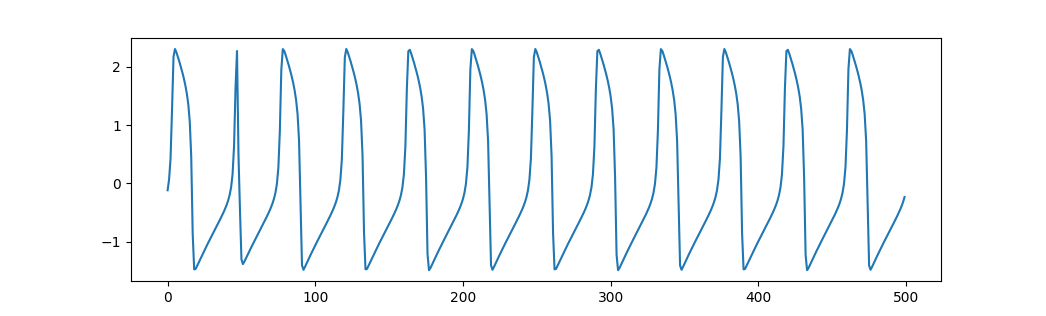
\includegraphics[width=0.9\linewidth]{fitzhughnagumo_sample.png}
%   \caption[
%     Sample time series based on the solution of the FitzHugh-Nagumo model
%   ]
%   {
%     Sample time series based on the solution $v(t)$ of the FitzHugh-Nagumo model, with parameters
%     $RI_{\mathrm{ext}}$ = 0.4, $\tau$ = 12.5, $a$ = 0.7, $b$ = 0.82.
%   }
%   \label{fig:fitzhughnagumo_sample}
% \end{figure}

The FitzHugh-Nagumo oscillator $v(t)$ is defined as a solution of the system:

\begin{equation}
  \begin{aligned}
    \ndif{v}{t} &= v - \frac{v^3}{3} - w + RI_{\mathrm{ext}} \\
    \tau \ndif{w}{t} &= v + a - bw
  \end{aligned}
  \label{eq:fhn}
\end{equation}

where $RI_{\mathrm{ext}}$, $\tau$, $a$, and $b$ are constant parameters to be determined.
%Fig.\ \ref{fig:fitzhughnagumo_sample} shows an example.

\pagebreak

In addition, I emulated noise by generating Gaussian and Gillespie noise.

Gaussian noise was generated by randomly drawing samples from the normal distribution $\mathcal{N}(0,\sigma^{2})$.
Here, $\sigma$ denotes the standard deviation of the distribution and thus controls the size of the noise.

% \begin{figure}
%   \centering
%   \begin{subfigure}{0.4\textwidth}
%     \centering
%     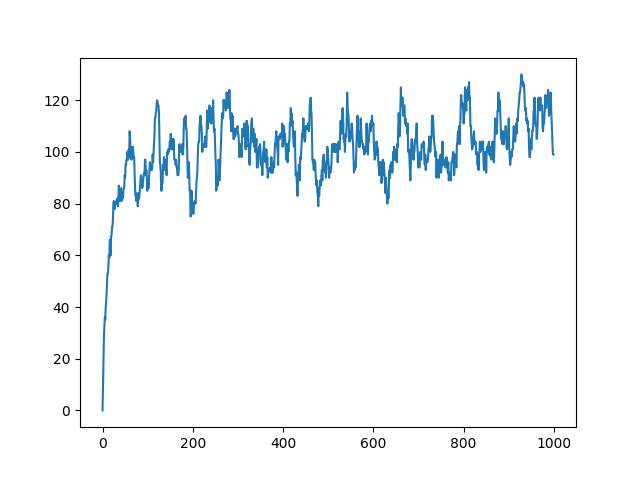
\includegraphics[width=\linewidth]{gillespie}
%     \caption{
%     }
%     \label{fig:gillespie_trajectory}
%   \end{subfigure}%
%  \begin{subfigure}{0.6\textwidth}
%     \centering
%     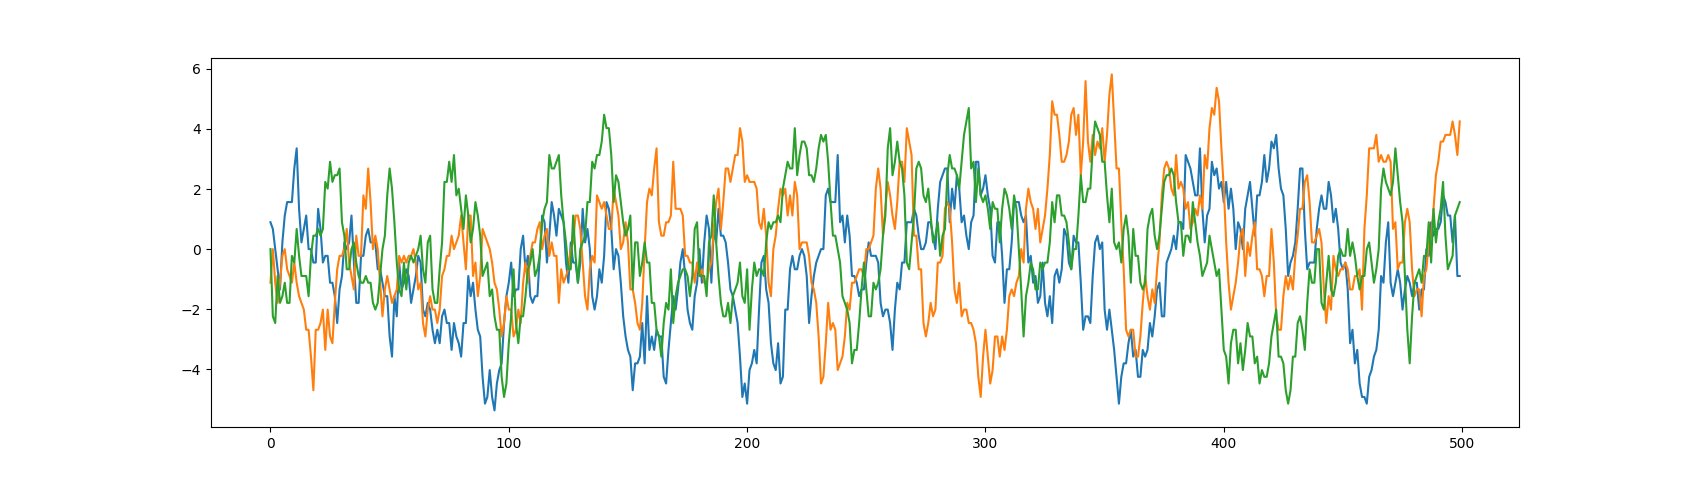
\includegraphics[width=\linewidth]{gillespie_noise_samples}
%     \caption{
%     }
%     \label{fig:gillespie_noise_samples}
%   \end{subfigure}

%   \caption[
%     Sample trajectory from a birth-death process and sample time series of Gillespie noise.
%   ]{
%     \textbf{(\ref{fig:gillespie_trajectory})}
%     Sample trajectory of a substrate created and destroyed by the birth-death process, simulated by the Gillespie algorithm ($k_{0} = 5$, $d_{0} = 0.05$, $t_{\mathrm{max}} = 1500$).
%     \textbf{(\ref{fig:gillespie_noise_samples})}
%     Sample time series of Gillespie noise, derived from trajectories generated as in (\ref{fig:gillespie_trajectory}).
%   }
%   \label{fig:gillespie_noise}
% \end{figure}

Gillespie noise emulates noise from biological systems.
Gillespie noise was generated using the direct method of the Gillespie algorithm \parencite{gillespieExactStochasticSimulation1977} on the birth-death process model (Appendix~\ref{append:analysis-gillespie}).

The birth-death process is a simple stochastic model used for the modelling of gene expression.
The model describes a species that is produced at a linear birth rate $k_{0}$ and destroyed at a linear death rate $d_{0}$, and is defined by the system of equations Eq.\ \ref{eq:birth-death-process}:

\begin{equation}
  \begin{aligned}
    R_{1}: \varnothing \ce{ &->[k_{0}] P}\\
    R_{2}: \ce{P &->[d_{0}]} \varnothing
  \end{aligned}
  \label{eq:birth-death-process}
\end{equation}

To produce Gillespie noise, a stochastic simulation employing the direct method of the Gillespie algorithm was performed on the birth-death process model with defined $k_{0}$ and $d_{0}$ parameters.
The final time was defined in such a way that allows the trajectory of the amount of $P$ over time to reach a steady state (Fig.\ \ref{fig:gillespie_trajectory}).
This time varied depending on the $k_{0}$ and $d_{0}$ values, but the final time of \num{1500} was chosen as it was long enough to have the trajectory reach steady state for the $k_{0}$ and $d_{0}$ values used in this study.

The latter half of the trajectory was taken and then put on a grid with \num{1000} regularly-spaced time points, equal to the number of time points for the synthetic oscillators (harmonic and FitzHugh-Nagumo).
The time series was then normalised by subtracting the mean ($k_{0}/d_{0}$) and then dividing by $\sqrt{1/d_{0}}$ to create a time series representing Gillespie noise with mean 0 and standard deviation $\sqrt{k_{0}}$.
This Gillespie noise thus has a standard deviation of noise amplitude $A = \sqrt{k_{0}/d_{0}}$ and noise timescale $\tau = 1/d_{0}$ --- in other words, the rate parameters of the birth-death process control the noise properties of this Gillespie noise.


\subsection{Signal-to-noise ratio}
\label{subsec:methods-computational-snr}

To evaluate the quality of oscillatory time series in a dataset and to indirectly measure the amplitude of the oscillations, I computed a signal-to-noise ratio for each time series.
%Because the information about the amplitude of the oscillations was removed when they were filtered using the high-pass Butterworth filter, a different measure is needed.
Assuming a constant noise introduced by the combination of intrinsic noise (stochasticity in biochemical processes) and extrinsic noise (variations introduced by measurement instruments), a low signal-to-noise ratio suggests a low oscillation amplitude, and the reverse is true for a high signal-to-noise ratio.

The signal-to-noise ratio can be defined as follows:

Given a time series $x(t) = x(t_{1}), x(t_{2}), \ldots, x(t_{N})$, the normalised classical periodogram (Fourier spectrum) is given by

\begin{equation}
  P(\omega) = \frac{N}{2\sigma^{2}} \left|\int_{-\infty}^{\infty} x(t) e^{-2\pi it}dt \right|, % check constants, etc
  \label{eq:normalised-periodogram}
\end{equation}

where $N$ is the number of time points in $x$ and $\sigma^{2}$ is the sample variance of $x$.
The periodogram $P$ is defined as a function of the angular frequency $\omega$.

A critical frequency $\omega_{c}$ is then defined to divide signal and noise --- that is, very high-frequency components of the periodogram correspond to noise and lower-frequency components correspond to the meaningful oscillations.

\pagebreak

The signal to noise ratio $r_{s/n}$ (Fig.\ \ref{fig:analysis-snr}) is thus defined as

\begin{equation}
  r_{s/n} = \frac{s}{n}
  \label{eq:snr}
\end{equation}

where the signal $s$ is defined as

\begin{equation}
  s = \int_{0}^{\omega_{c}} P(\omega) d\omega
  \label{eq:signal}
\end{equation}

and the noise $n$ is defined as

\begin{equation}
  n = \int_{\omega_{c}}^{\infty} P(\omega) d\omega
  \label{eq:noise}
\end{equation}


\begin{figure}[hb!]
  \centering
  \begin{subfigure}[htpb]{0.5\textwidth}
   \centering
   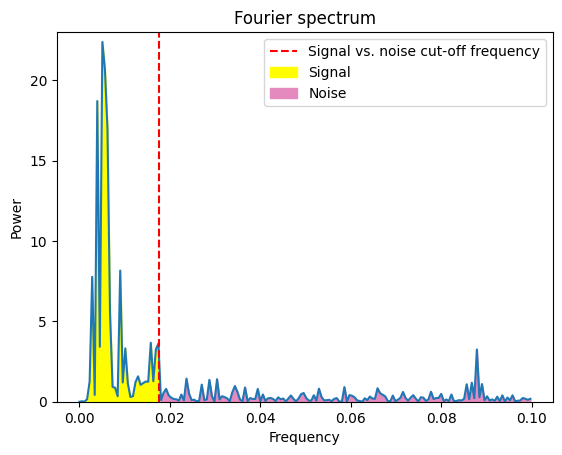
\includegraphics[width=\textwidth]{snr_illustration}
   \caption{
   }
   \label{fig:analysis-snr-illustration}
 \end{subfigure}%
 \begin{subfigure}[htpb]{0.5\textwidth}
   \centering
   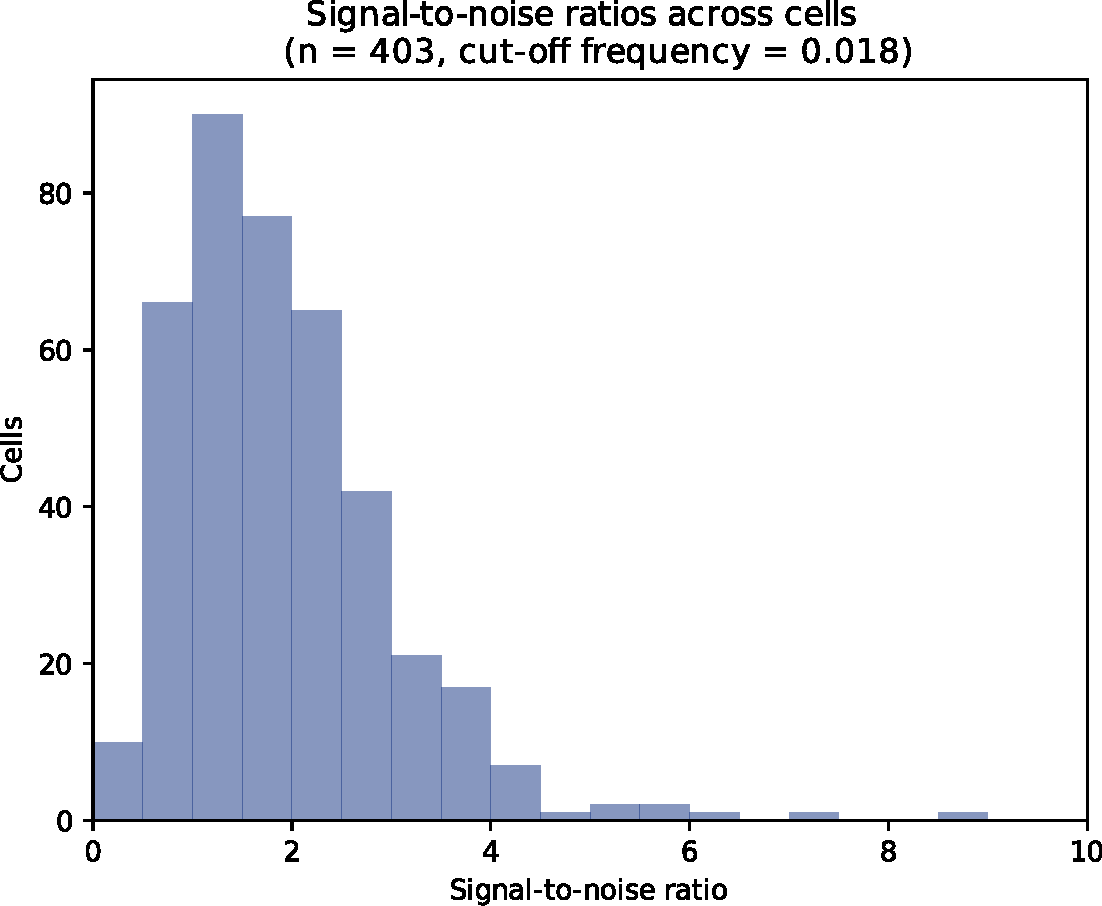
\includegraphics[width=\textwidth]{pyruvate_snr_edit}
   \caption{
   }
   \label{fig:analysis-snr-histogram-example}
  \end{subfigure}

  \caption[
    Illustration of signal-to-noise ratio.
  ]{
    %The signal-to-noise ratio as a measure of signal quality.
    \textbf{(\ref{fig:analysis-snr-illustration})}
    Illustration of signal-to-noise ratio.
    The signal-to-noise ratio is defined (Eqs.\ \ref{eq:normalised-periodogram}--\ref{eq:noise}) as the area under the periodogram below a cut-off frequency (yellow) divided by the area under the periodogram above a cut-off frequency (pink).
    \textbf{(\ref{fig:analysis-snr-histogram-example})}
    Histogram of signal-to-noise ratios from a sample experiment ($n=403$).
  }
  \label{fig:analysis-snr}
\end{figure}

In this thesis, I define $\omega_{c} = \SI{0.018}{\minute^{-1}}$, corresponding to a period of \SI{55}{\minute}, because this period is smaller than the periods of all oscillations of flavin autofluorescence I observed in my experiments.


\section{Methods related to flux balance analysis}
\label{sec:methods-fba}

To evaluate biosynthesis strategies in the \textit{S. cerevisiae} cell, I used the ecYeast8 \parencite{luConsensusCerevisiaeMetabolic2019} genome-scale metabolic model and performed flux balance analysis.

\subsection{ecYeast8 formalisms}
\label{subsec:methods-fba-ecYeast8}

The formalisms used in ecYeast8 differ from the usual formalisms used in genome-scale metabolic models.
ecYeast8 contains four formalisms relevant to this thesis:
\begin{enumerate}
  \item
        The biomass reaction is defined by having `pseudometabolites' as reactants and a biomass species as a product.
        These pseudometabolites include lipids, proteins, carbohydrates, RNA, DNA, ions, and cofactors.
        This is in contrast to BiGG genome-scale models \parencite{norsigianBiGGModels20202020}.
        In these models, biomass reactions have chemical species as reactants, and each has a stoichiometric coefficient that is equal to the species' abundance in units of \SI{}{\mmolgdw}.
  \item
        The pseudometabolites are defined by `\textit{isa}' reactions, which group specific chemical species into classes of metabolites \parencite{heavnerYeastExpandedReconstruction2012}.
        These reactions account for how some KEGG definitions of reactions require generic compounds and these reactions also allow flexibility of biomass definition in different growth conditions.
        The \textit{isa} reactions have chemical species as reactants, each with a stoichiometric coefficient representing the species' abundance in units of \SI{}{\mmolgdw}, and a pseudometabolite as a product.
        In effect, the species abundance information is shifted one reaction away from the biomass reaction.
  \item
        The models implements SLIMEr \parencite{sanchezSLIMErProbingFlexibility2019}, which Splits Lipids Into Measurable Entities, and adds constraints on lipid classes and acyl chain distribution.
        This formalism is needed because species of lipid backbones and acyl chain can combine to form lipids in more than a thousand ways, and the resulting lipid species are difficult to all be represented in a genome-scale metabolic model.
        SLIMEr thus introduces reactions that split lipids into their basic components and lipid pseudoreactions to preserve the distribution of acyl chains.
        As a result, the definitions of lipids are flexible.
  \item
        GECKO \parencite{sanchezImprovingPhenotypePredictions2017} was applied to Yeast8 to produce ecYeast8.
        GECKO modifies the stoichiometric matrix of a genome-scale metabolic model to account for enzyme abundances and kinetics.
        Specifically, it adds to enzyme-catalysed reactions enzyme species with a stoichiometric coefficient derived from its $k_{cat}$ value.
        The formalism also adds reactions to model drawing enzymes from a pool.
        GECKO simulates an upper limit of amino acids available for enzyme production.
\end{enumerate}


\subsection{Computing molecular weights of pseudometabolites}
\label{subsec:methods-fba-molweights}

To compute the synthesis time for each biomass component, the mass fractions of each biomass component must be known.
These quantities are typically stored as molecular weights in a genome-scale model.
As biomass components in ecYeast8 are pseudometabolites without specified molecular weights, I computed the mass fractions of each biomass component based on their \textit{isa} reactions (Appendix~\ref{append:model-molweights}).
Rather than using mass fractions based on experimental studies, I used mass fractions based on the model because the mass fraction of each biomass component varies according to strain and growth rate \parencite{nilssonMetabolicTradeoffsYeast2016, elsemmanWholecellModelingYeast2022}.

Table~\ref{tab:ecyeast8-mol-weights} summarises the molecular weight of the pseudometabolites.
The ratio between the molecular weights are similar to the ratio between the mass of each class of macromolecule in the yeast cell dry weight shown by \textcite{canelasVivoDatadrivenFramework2011}, thus validating my calculations.

\begin{table}[ht]
  \centering
  \begin{tabular}{lSS}
    \toprule
    Metabolite & {\makecell{Computed molecular weight\\ (\SI{}{\gram~\mol^{-1}})}} & {\makecell{Biomass composition\\ at growth rate \SI{0.375}{\hour^{-1}}\\ (\SI{}{\gram~\kilo\gram_{DW}^{-1}})}} \\
    \midrule
    Protein & 504.37 & 505.\\
    Carbohydrate & 350.37 & 237.\\
    RNA & 64.04 & 105.\\
    Lipid & 31.57 & 57.\\
    Cofactors & 4.83 & \\
    DNA & 3.90 & 5. \\
    Ions & 2.48 & \\
    \bottomrule
    Total & 961.57 & \\
  \end{tabular}
  \caption[
    Computed molecular weights of bulk metabolites in ecYeast8, compared to experimentally recorded biomass composition
  ]{
    Computed molecular weights of bulk metabolites in ecYeast8, compared to experimentally recorded biomass composition by \textcite{canelasVivoDatadrivenFramework2011}.
  }
  \label{tab:ecyeast8-mol-weights}
\end{table}

Adding together molecular weights of pseudometabolites gave a molecular weight of the biomass pseudometabolite of \SI{961.57}{\gram~\mol^{-1}}, close to the \SI{966}{\gram~\mol^{-1}} computed by \textcite{takhaveevTemporalSegregationBiosynthetic2023} from a different genome-scale model.
In theory, this number should be \SI{1000}{\gram~\mol^{-1}} because the stoichiometric coefficients of the species that form biomass components are expressed in terms of \SI{}{\mmolgdw} \parencite{thieleProtocolGeneratingHighquality2010, palssonSystemsBiologyConstraintbased2015}, but the deviation from 1000 could be explained by the SLIMEr formalism.
In addition, the sum of stoichiometric coefficients is not always verified in genome-scale models \parencite{chanStandardizingBiomassReactions2017}.

%%% Local Variables:
%%% mode: latex
%%% TeX-master: "../thesis.tex"
%%% End:
